\chapter{\label{chap:state-of-the-art}State of the Art}
% Gnutella, Scuttlebutt, libp2p -> possible additions, but not really necessary
In this chapter we describe existing algorithms, protocols and applications in computer science, which try to solve, or give an alternative for, the centralized power on Internet platforms, and more specifically in digital audio streaming. We analyze state-of-the-art algorithms and protocols that can be used to implement components of our robot economy framework. Additionally, we review recent decentralized music streaming applications.

For an application to evolve in a fully distributed network, without a company or a single point of responsibility, decisions need to be made on protocol or feature additions and changes. We inspect the state-of-the-art technologies and organizational theories which enable autonomous communities to solve these problems by organizing themselves.

\section{Decentralized Autonomous Organizations}
\label{sec:dao}
As an alternative organizational framework for distributing money and music, we examine a recent theory in distributed systems research: a Decentralized Autonomous Organization (DAO).
A DAO is ``an entity that lives on the internet and exists autonomously, but also heavily relies on hiring individuals to perform certain tasks that the automaton itself cannot do''~\citep{buterin2014dao}. It is not owned by a single person or legal entity. It should also not require a specifically specified party to operate. For example, it should not depend on a single server or database, but rather have flexibility in adopting resources. As such we say it lives \textit{autonomously}. \cite{buterin2014dao} also notes that a DAO should have \textit{internal capital}: ``some kind of internal property that is valuable in some way, and it has the ability to use that property as a mechanism for rewarding certain activities''. A DAO is non-profit by nature, as there is no legal owner of the system.

% Add The DAO example/add example of shared wallet system

Important groundwork on the theory and implementation of a DAO has been done by \cite{jentzsch2016decentralized}. He notes that corporations originally work through people only, and this has two flaws: ``People do not always follow the rules, and they do not always agree what the rules require''. His paper illustrates a method that allows creating and maintaining organizations in which ``(1) participants maintain direct real-time control of contributed funds and (2) governance rules are formalized, automated and enforced using software''.

\section{AI and DAO}
The combination of intelligent agents and DAO technologies allows building an autonomous, decentralized and self-evolving software system. This may present the first ingredients towards a robot economy in software. In a system on the boundary of DAO and artificial intelligence (AI) technologies, humans are still involved with performing some tasks and governing, but intelligent agents can perform other decision making tasks on their own. Decision making by robots can be done using a wide range of state-of-the-art algorithms and techniques shown in fig. \ref{fig:ai-techniques}.

One implementation of intelligent agents acting autonomously is CloudOMate~\citep{jaspers2018plebnet}. This is a software system that runs autonomously and is self-replicating: it can extend its network infrastructure on its own by contacting hosting companies. This can be connected to an AI algorithm which learns when an expansion of network resources is necessary. It has internal capital that is used to pay service fees to hosting providers.

\begin{figure}
    \centering
    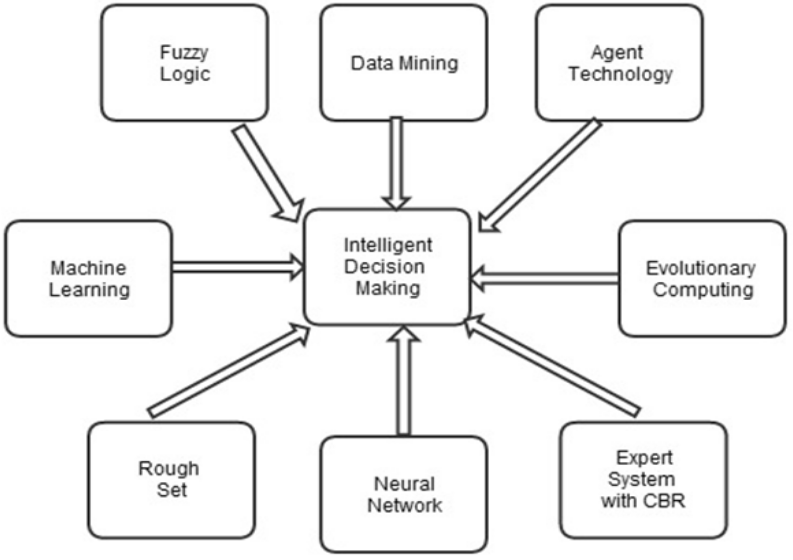
\includegraphics[width=0.5\textwidth]{related-work/intelligent-decision-making.png}
    \caption{Intelligent techniques in decision making (source:~\cite{das2016intelligent})}
    \label{fig:ai-techniques}
\end{figure}

In our context, we envision human tasks to be e.g. (1) creating music and giving feedback on music (through e.g. donations), (2) making decisions on the subscription protocol and the payouts to artists, or (3) governing evolution of the software. \textit{Robot tasks} could be e.g. (1) processing an automatic subscription payment system, in which all user money is divided fairly over the artists every time iteration, (2) tracking connectivity stats of other users, or (3) determining trust of authenticity and identity of artists.

% Move to Design
% Much is still unknown in this research area. This thesis aims to create more knowledge on a 'AI DAO' by attempting to build a proof-of-concept of such intelligent system.

\begin{figure}
    \centering
    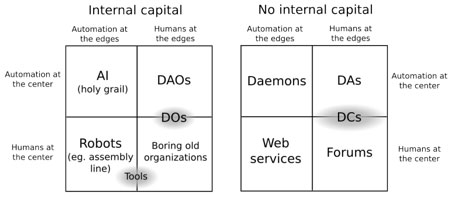
\includegraphics[width=0.7\textwidth]{introduction/dao-quadrants.jpg}
    \caption{Decentralized Autonomous Organization, in comparison to other organizational structures. In a DAO, activity is performed by humans at the edges, automation at the center. It is an interplay in which robots and humans perform tasks. Source: \cite{buterin2014dao}}
    \label{fig:dao-quadrants}
\end{figure}

\section{Decentralized music distribution technologies}
\label{sec:related-work}
There exist a few recent decentralized audio distribution and streaming applications exist. The most notable examples are Audius~\citep{audius2018}, Musicoin~\footnote{\url{http://musicoin.org/}} and Opus Audio~\citep{jia2016opus}.

Audius~\citep{audius2018} presents a decentralized protocol for audio content, which aims to improve payouts to artists and its transparency. It contains a token economy with a transparent payout system for the artists, and a user-operated, distributed network for metadata and content. Its monetary infrastructure is displayed in fig. \ref{fig:monetary-flow-audius}. In addition, it has a governance system like a DAO, in which users can decide on changes to the protocol by democratic voting. Its protocol is established around the ideology of disintermediation: ``Intermediaries  should be removed  when possible; when necessary, they should be algorithmic, transparent, and verifiably accurate''~\citep{audius2018}. It uses IPFS~\citep{benet2014ipfs} for storage of audio content.
% The last sentence is most likely not true

Opus Audio~\citep{jia2016opus} is a decentralized music-sharing protocol and platform and describes a solution for music ownership registration on a blockchain structure. It has an operational distributed audio file sharing system using IPFS \cite{benet2014ipfs} (see \ref{sec:decentralized-content-delivery}). It contains a decentralized and fully automated system for purchasing access to music, which works as follows. Opus stores encrypted audio files on a swarm of connected nodes. The decryption keys and files hashes are stored in a smart contract (see \ref{sec:smart-contracts}). Using cryptocurrency, users spend their funds on these smart contracts, to unlock access to audio files, and to cooperate in its permissionless DAO (see fig. \ref{fig:opus-dao}).

\begin{figure}
    \minipage{0.4\textwidth}
        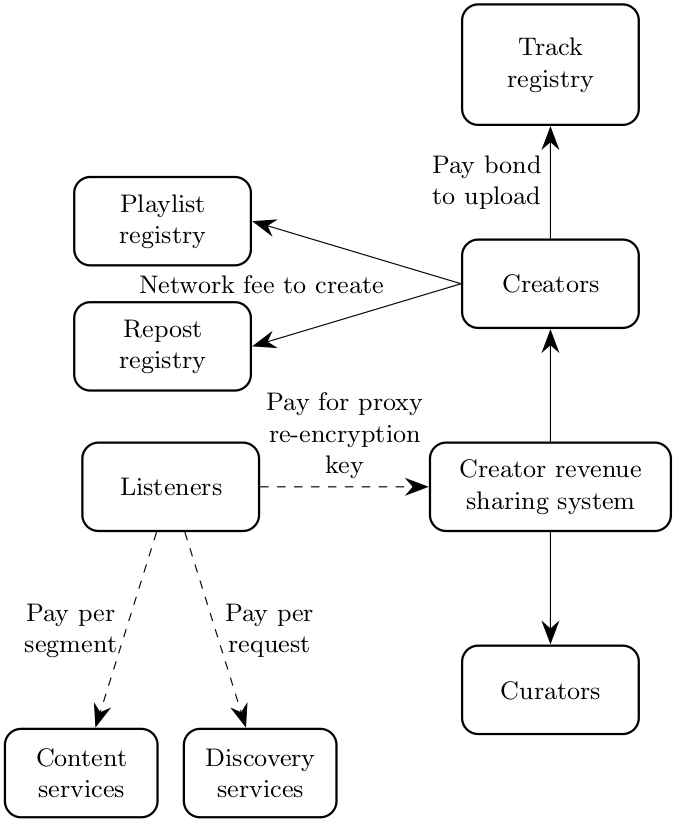
\includegraphics[width=1\linewidth]{related-work/audius-money-flow.png}
        \caption{Monetary flow in Audius (source:~\cite{audius2018})}
        \label{fig:monetary-flow-audius}
    \endminipage\hfill
    \minipage{0.5\textwidth}
        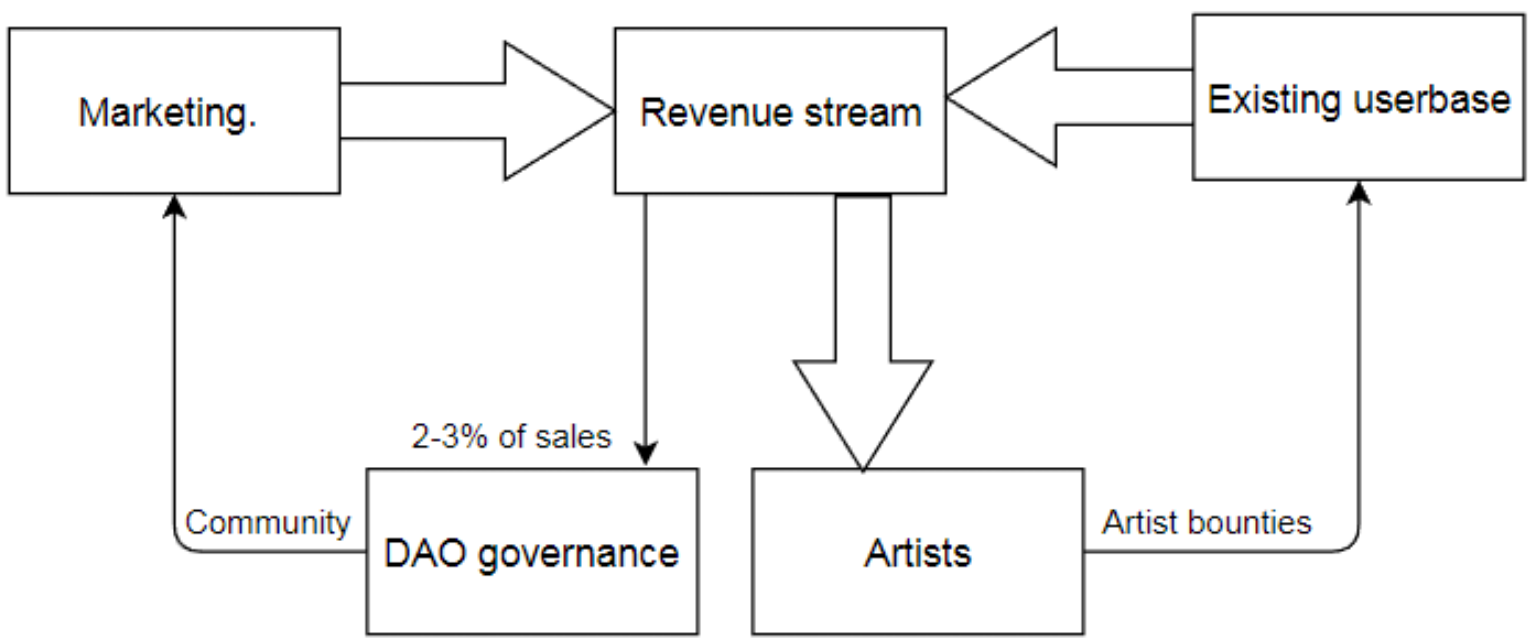
\includegraphics[width=1\linewidth]{related-work/opus-dao.png}
        \caption{Effect of DAO governance system on revenue streams in Opus (source:~\citep{jia2016opus})}
        \label{fig:opus-dao}
    \endminipage
\end{figure}

Musicoin is a blockchain platform without intermediaries that focuses on income for independent artists. It uses smart contracts and cryptocurrency to show transparency in payments (see \ref{sec:smart-contracts}). This payment structure ensures that each contributor in the network is rewarded, and that artists receive a stable income based on the Universal Basic Income ideology. Not all of their architecture is decentralized; they use centralized registration system for artists and listeners. They pay artists using their \$MUSIC currency, of which the value may be highly volatile.

None of the state-of-the-art decentralized audio streaming technologies show a running, fully decentralized or self-scaling infrastructure with stable income for artists. All of these systems have in common that they save metadata and identifiers of audio files on a blockchain, and save the audio files in an off-chain database using IPFS~\citep{benet2014ipfs}. This makes these solutions reliant on people voluntarily running IPFS content nodes (servers hosting the audio files). In a fully decentralized network, every participant should have the same role, meaning that every node both uploads and downloads content, and it should not be reliant on external servers. Additionally, all of these technologies use their homebrew cryptocurrency to pay artists, instead of a stable currency.

\section{Financial transparency in the music industry}
\label{sec:smart-contracts}
As described in sec. \ref{sec:problem-financial-transparency}, there is a serious issue in the music industry affecting artists globally: the (by design) inaccurate, complex and slow royalty payments. There are existing decentralized frameworks and protocols to solve this problem.

Payments of royalties to artists can be described in transparent, public and immutable records on a blockchain. In addition, smart contracts can be used to automate payments~\citep{buterin2014next}. Smart contracts are self-executing (non-ambiguous) and self-verifying (guaranteeing its statements). In the music industry context, a smart contract can be used for transparent, immutable and automatic payment distribution of royalties. This technique was shown in practice in 2017, when Imogen Heap released the song `Tiny Human'~\citep{heap2017blockchain}. Its distribution of payments to the makers and recorders was written in a smart contract, in the form of a record on the Ethereum blockchain. When a user downloads the corresponding track and makes the payment using cryptocurrency, the forwarding details of the payment are located within the blockchain, and executed as declared on the smart contract, on a distributed virtual machine (VM) such as the Ethereum VM.

% \section{Distributed ledger technology}
% A distributed ledger is a technology used to create data stores in a distributed network. 
% Expand, explain TrustChain

\section{Decentralized application frameworks}
% Add at least one or more decentralized application frameworks
% Add a good intro: why do we need a Decentralized App Framework?
\label{sec:sote-trustchain}
There exist decentralized application frameworks which assist in creating peer-to-peer technologies. A suitable software framework to use for building an alternative for Big Tech is the TrustChain Superapp. The TrustChain Superapp~\citep{mattskala2020} is a framework for implementing mobile Android decentralized applications. It allows for storing append-only immutable data on TrustChain~\citep{otte2017trustchain} and spreading this data in a phone-to-phone network without servers. It follows the concept of super apps~\citep{kpmg2019superapps}, meaning that it contains many mini-apps which use the same networking interface. The Superapp is an Android app as seen in fig. \ref{fig:trustchain-superapp}. Its mini-apps implement distributed democratic voting and has bitcoin payment integration, among other features.

\begin{figure}
    \minipage{0.3\textwidth}
        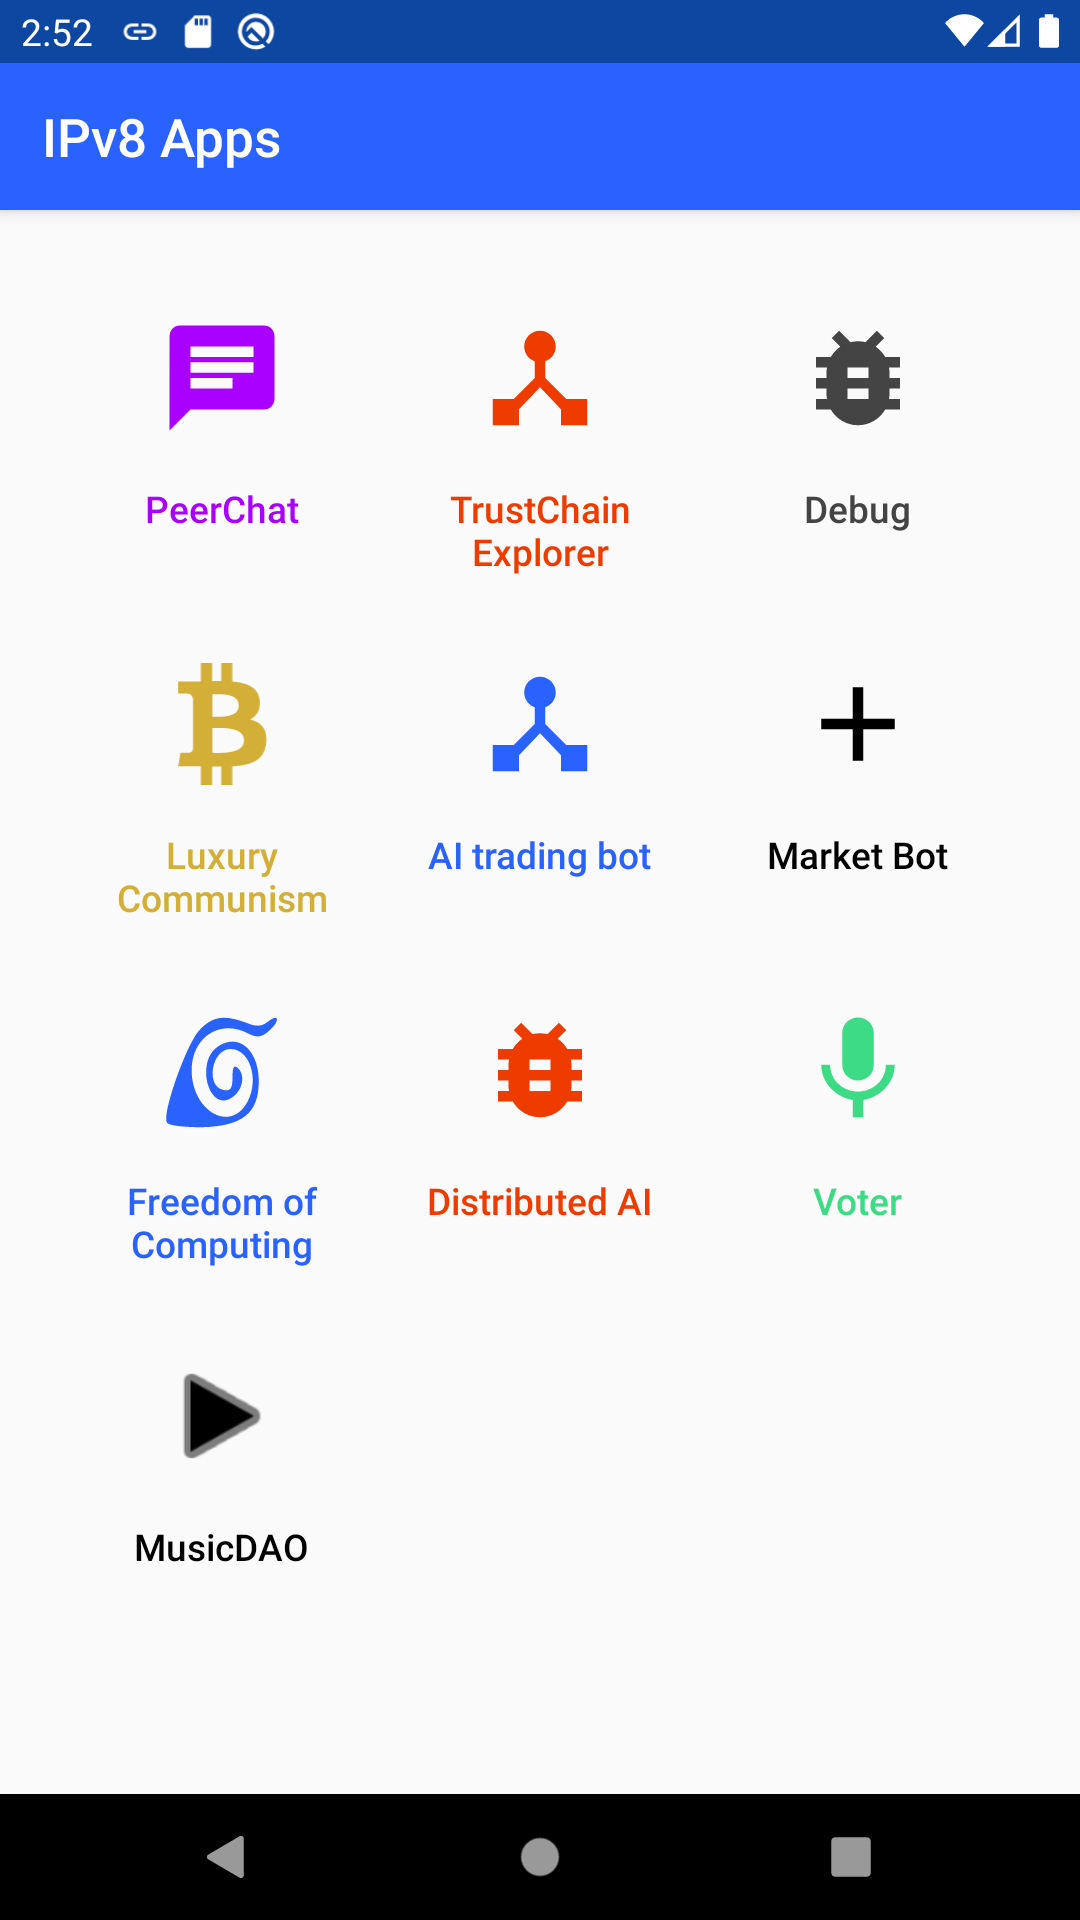
\includegraphics[width=1\linewidth]{related-work/screenshot-superapp.png}
        \caption{Trustchain-Superapp overview}
        \label{fig:trustchain-superapp}
    \endminipage\hfill
    \minipage{0.65\textwidth}
        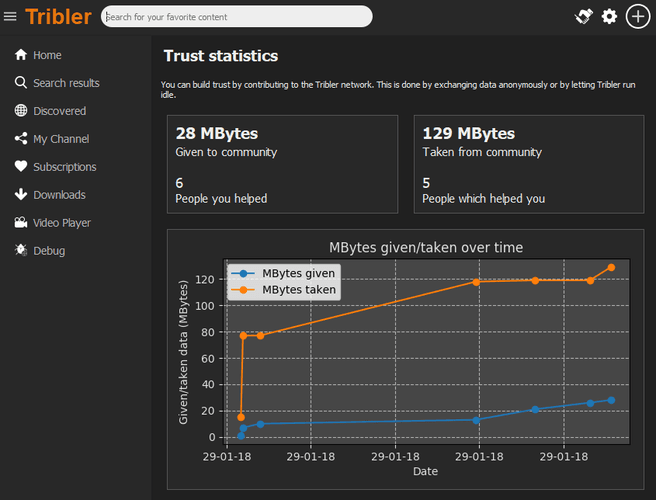
\includegraphics[width=1\linewidth]{related-work/tribler7.3.0.png}
        \caption{Tribler desktop interface, showing the bandwidth incentive system overview}
        \label{fig:tribler}
    \endminipage
\end{figure}

In the context of self-governance, the TrustChain Superapp contains an operational distributed governance protocol implemented as a distributed voting app (see fig. \ref{fig:trustchain-superapp-voter}). In this voting app, any participant of the organization can create a proposal for the community to vote on. Once a preset voting threshold is reached, the proposal is automatically accepted or denied. This voting app is an important basis for democratic decision making. It could be extended to include continuous, automated code evolution: by voting on code patches or changes, the community can decide on new features of the application. This protocol is based on proof-of-identity instead of proof-of-stake, as no tokens are involved.

\begin{figure}
    \centering
    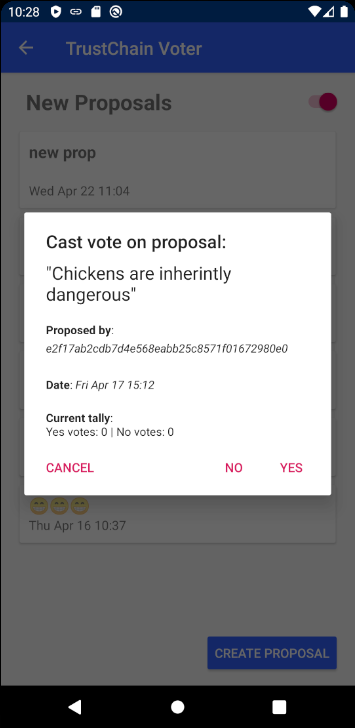
\includegraphics[width=0.3\linewidth]{related-work/trustchain-superapp-voter.png}
    \caption{\textit{Distributed democracy} voting mini-app, showing proposals}
    \label{fig:trustchain-superapp-voter}
\end{figure}

% Add MakerDAO

\section{Decentralized content delivery networks}
\label{sec:decentralized-content-delivery}
A fully decentralized audio streaming service requires sharing and streaming audio files over a network of nodes in which any participant can start and run a node. Well-established examples of such technologies are BitTorrent and IPFS.

\subsection{BitTorrent}
\label{sec:sote-bittorrent}
BitTorrent~\citep{cohen2002bittorrent} is an open peer-to-peer file sharing protocol. It was invented by Bram Cohen, and has generated a massive influence on network traffic on the Internet since its release. Today, it is still the most popular peer-to-peer protocol for sharing data. In 2019, BitTorrent was measured to generate 2.5\% of all download and 24.6\% of all upload bandwidth~\citep{marozzo2020}. It went through many iterations and improvements. It has a large community, with over 3K repositories on GitHub related to the technology.

In essence, BitTorrent makes use of seeding while downloading: this means that when multiple clients download a file, they simultaneously share pieces of this file with the other downloaders. This results, with well connected and performing peers, in fast downloads. BitTorrent originally relied on trackers to perform peer discovery, and trackers can become a central point of failure. However, since the introduction of the DHT protocol~\citep{bittorrentbep5dht}, finding peers in the network can be done by querying any known peer, which makes the network more decentralized. 

% Any person can join the network and start sharing files, by making a torrent which contains the metadata of the files. Content is specified using SHA1 hashes of the files. Checksums are used to make sure no changes to the original torrent have been made upon receiving files. This way all files are immutably shared. BitTorrent has implementations for various systems, including Android. This means mobile devices can participate in uploading and downloading content, and can even build an autonomous phone-only file sharing system.

% Torrent files contain a list of chunks (torrent pieces), which represent the different parts of the related file. Flawless streaming of media files over BitTorrent requires a smart algorithm to predict what file is requested next, and what torrent pieces should be loaded. 

There are no differences between hosters and downloaders. All participants have the same capabilities, so every user of the network can both download and upload content. It uses tit-for-tat as a method of efficiently downloading files. However, an open problem in BitTorrent is incentivizing participants to host files. There are multiple proposed solutions for this, discussed in \ref{sec:file-spreading-incentives}. 
\subsection{IPFS}
The Inter-Planetary FileSystem (IFPS), introduced by \cite{benet2014ipfs}, is a distributed peer-to-peer file sharing system in which any person can start a node and start uploading and downloading files. Protocol Labs\footnote{\url{https://protocol.ai/}}, the team behind this technology, was founded in 2014 by Juan Benet. As of 2020, the team has grown globally to members from 19 countries, with substantial investments. However, there has not been large-scale adoption of this technology yet.

% It uses a Distributed Hash Table to address content using a combination of SHA-256 hashes and hyperlinks. 

At its core, IPFS maintains a global key-value store for all files (and file parts). This is in contrast to BitTorrent, which works with torrent swarms and trackers. IPFS uses an efficient content addressing mechanism. Another feature is built-in file de-duplication. Additionally it supports public file history bookkeeping.

End-users of content stored on IPFS can access content without supporting the network, so there is the possibility of free-riding. In addition, there are no direct (financial) incentives to run an IPFS node, other than to support the network. 
% For example, users of the aforementioned Audius music streaming system are not required to run an IPFS node to improve the health of the network. 
% \subsection{Comparison: IPFS and BitTorrent}
\\
\\
When comparing IPFS and BitTorrent, a notable difference between IPFS and BitTorrent is that IPFS makes a distinction between file-hosting nodes and end-users (which only download files). BitTorrent does not make a distinction between these actors. In BitTorrent, every participant of the network has the capabilities to both upload and download content. Therefore a BitTorrent network using DHT is typically more decentralized than IPFS. 

IPFS uses a global file index using a hash tree, which means that every two files that produce the same hash are stored on the same index. This leads to de-duplication, which may result in better use of disk space, in comparison to BitTorrent.

\section{File hosting incentive algorithms}
\label{sec:file-spreading-incentives}
In a decentralized network, determining the entity responsible for hosting files is not trivial. To tackle the tragedy of the commons, participants should have an incentive to contribute their computational and bandwidth resources to the network, so that it is responsive. One example incentive system is bandwidth tokens~\citep{de2018blockchain} as part of the Tribler system. Another is FileCoin: a decentralized storage network that rewards uploaders of content in terms of tokens.

Tribler~\citep{pouwelse2008tribler} is a peer-to-peer system to share, download and stream multimedia. It has implementations for desktop environments and an Android prototype. It makes use of BitTorrent for file transfer and adds anonymization techniques on top of it. In addition, it makes use of its bandwidth tokens: an incentive system to increase cooperation between users, in order to achieve high availability of downloads. In essence, it subtracts tokens for downloading content from peers and rewards tokens for helping peers. An overview of the Tribler desktop interface, showing this tit-for-tat protocol in operation, can be seen in fig. \ref{fig:tribler}.

FileCoin~\citep{benet2018filecoin} is an addition on top of the distributed file storage system IPFS. It is a distributed incentive protocol which rewards users for hosting files in the network. In essence, there is a decentralized market over which cryptocurrency (FileCoin) is transacted. Supply and demand of files in the network determine the reward value in terms of FileCoin. The mechanism for obtaining these coins is somewhat similar to the mining protocol in Bitcoin, but uses \textit{proof-of-storage} instead of \textit{proof-of-work} as a way to determine block rewards.

% \section{Distributed Ledger Technologies}